\section{GameManager}
Die Klasse GameManager ist zuständig für Training und Evaluation der Agenten sowie das Logging.
In \cref{fig:uml_sequence} ist der vereinfachte Ablauf des Trainings mit klassischem \splay für AgentSARSA dargestellt.
Für jedes Training wird ein neues Gamefield erzeugt und Experimentparameter definiert, auf deren Basis Experience und Agenten initialisiert werden. 
Zu Beginn jeder Episode werden die Hyperparameter der Agenten entsprechend der Experimentparameter aktualisiert. 
Anschließend wird ein Spiel gestartet und in jedem Zug werden der Zustand und die legalen Aktionen des Gamefields abgerufen. 
Beginnend mit X werden abwechselnd die move-Methoden der Agenten aufgerufen, in dessen Rahmen der direkte Reward, $r=0$, ausgegeben wird. 
Die zurückgegebene Aktion wird auf das Gamefield angewandt. 
Nach Ende des Spiels, wird der Reward mit Depth Penalty für die letzte Aktion beider Agenten verteilt und das Spielfeld zurückgesetzt. 
Das Training mit alternierendem \splay folgt dem gleichen Ablauf.
Innerhalb eines Batchs werden die Hyperparameter des nicht lernenden Agenten so gesetzt, das dieser mit der Greedy-Strategie spielt und bei Aufruf seiner move-Methode kein \ac{TD} Update durchführt.
Im Anschluss an das Training werden beide Agenten im Rahmen von Evaluationsspielen bewertet und die Experience Instanz wird als Datei serialisiert.

\begin{figure}[h]
    \centering
    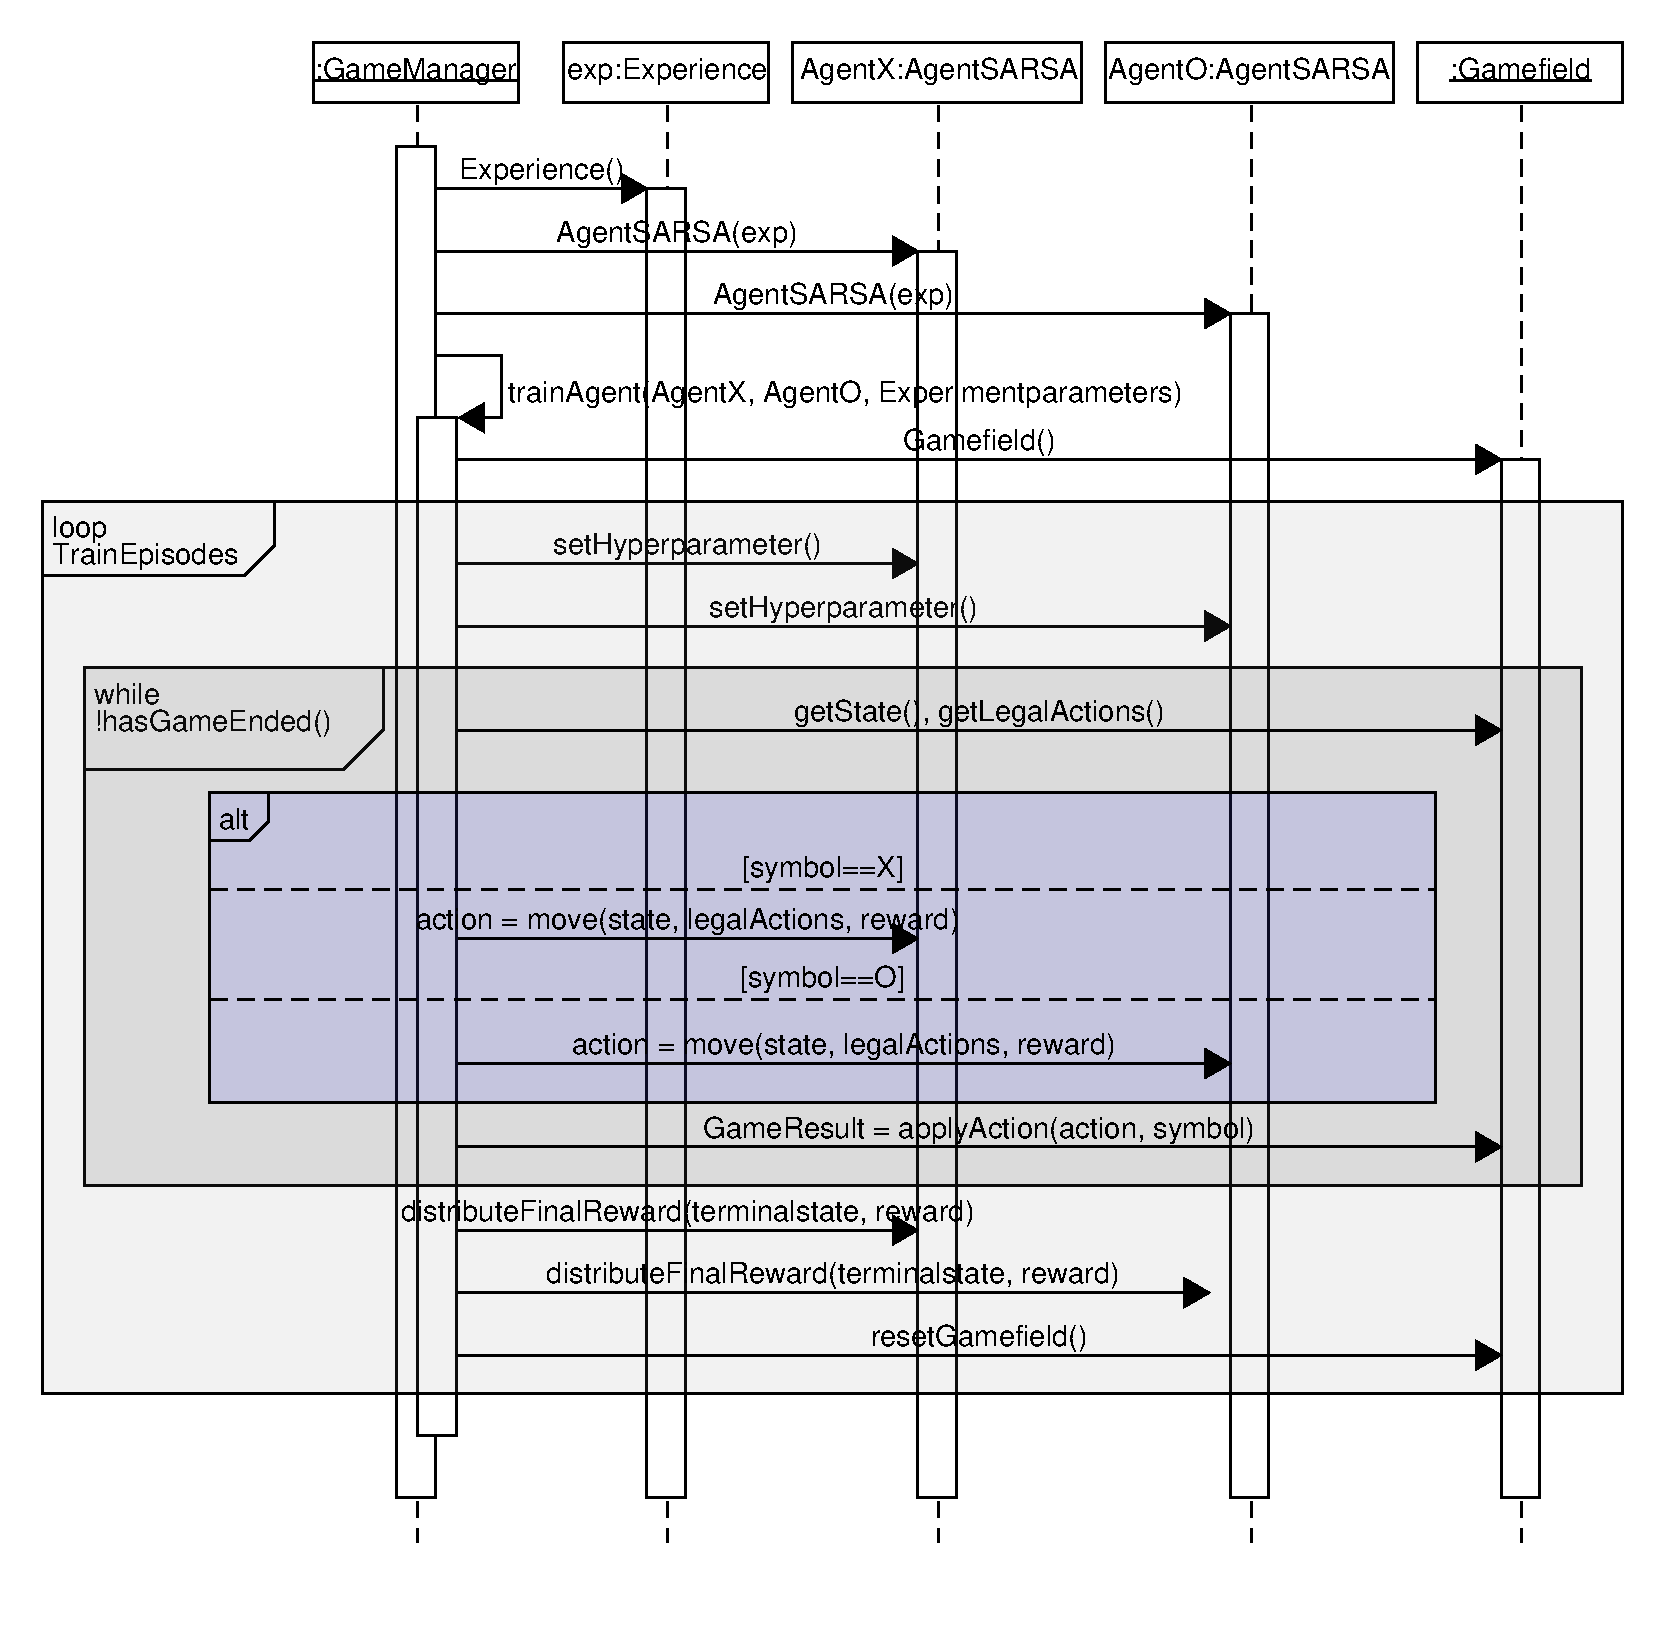
\includegraphics[width=\linewidth]{04_Artefakte/01_Abbildungen/uml/uml_sequence.pdf}
    \caption{Vereinfachte Darstellung des Trainingsablaufs mit klassischem \splay}
    \label{fig:uml_sequence}
\end{figure}